\documentclass[UTF8, 11pt, oneside]{ctexart}

\usepackage{float}

\usepackage{geometry}
\geometry{a4paper,left=2cm,right=2cm,top=2cm,bottom=1cm}

\usepackage{graphicx}

\usepackage{hyperref}
\hypersetup{colorlinks=true, linkcolor=red}

\linespread{1.6}


\def\articletitle{解放军把坦克大炮拉上渔船,只为对抗1996年的美军航母}

\usepackage{fancyhdr}
\usepackage{ifthen}
\pagestyle{fancy}
\fancyhf{}
\setlength{\headheight}{14pt}
\fancyhead[R]{\ifthenelse{\value{page}>1}{\thepage}{}}
\fancyhead[C]{\ifthenelse{\value{page}>1}{\articletitle}{}}
\renewcommand\headrulewidth{0pt}

\usepackage{tcolorbox}
\tcbuselibrary{skins}


\newcommand{\zd}[1]{\textbf{\textcolor[RGB]{123,12,0}{#1}}} % 重点

\newcommand{\yh}[1]{% 引用
    \begin{tcolorbox}[enhanced,
        frame hidden, interior hidden,
        before skip = 5mm, left skip=10mm,
        borderline west={5pt}{0pt}{gray!50}]
        #1
    \end{tcolorbox}
}

\newcommand{\biaoti}[1]{% 标题
    \section*{#1}
}

\begin{document}

\begin{center}
    \LARGE{\articletitle\footnotemark}
\end{center}
\footnotetext{
    原文出自公众号“远方青木”的文章 《\href{https://mp.weixin.qq.com/s/NlpDRhbVZV47eE0rMBFOsA}{\articletitle}》
}

1991年苏联解体,在确认苏联死透后,中美蜜月期直接结束。

因为没有苏联需要利用中国去遏制了,中国对美国而言价值急剧下降,从需要被拉拢的对象变成了需要被遏制的对象。

1993年,美国军舰无理由扣押中国“银河号”货轮强行检查,中国的军力无法对此进行反制。

1995年5月,台湾李登辉访美,打破了中美关系正常化以来的政治底线。

在李登辉的鼓吹和美国的支持下,台独思想开始急速蔓延,如果不对此进行遏制,为和平解放台湾而持续数十年的努力将可能付诸东流,台湾的民意将从倾向于和平解放,无法逆转的全面倒向台独。

1995年7月,中国进行了台海军演,在台湾海峡试射东风-15短程导弹6枚,出动舰艇200艘,出动飞机850架次,以此来震慑台独势力。

对此美国的反应是派出尼米兹号核航母战斗群,于1995年12月19日在台湾海峡航行,对中国耀武扬威,台独势力欢声震天。

为遏制台独势力,中国决定于1996年3月5日,联合海陆空三军,大规模调集军力,在台湾海峡再度进行军演。

这一次光陆军就派出了数十万人云集东南沿海,海空军几乎集中了全部力量,战略导弹部队全体战备。

\zd{1996年3月8日,美国下令尼米兹号核航母战斗群和独立号航母战斗群开赴台湾海峡,和中国海军形成对峙。}

\zd{96年台海危机正式爆发。}

\begin{figure}[H]
    \centering
    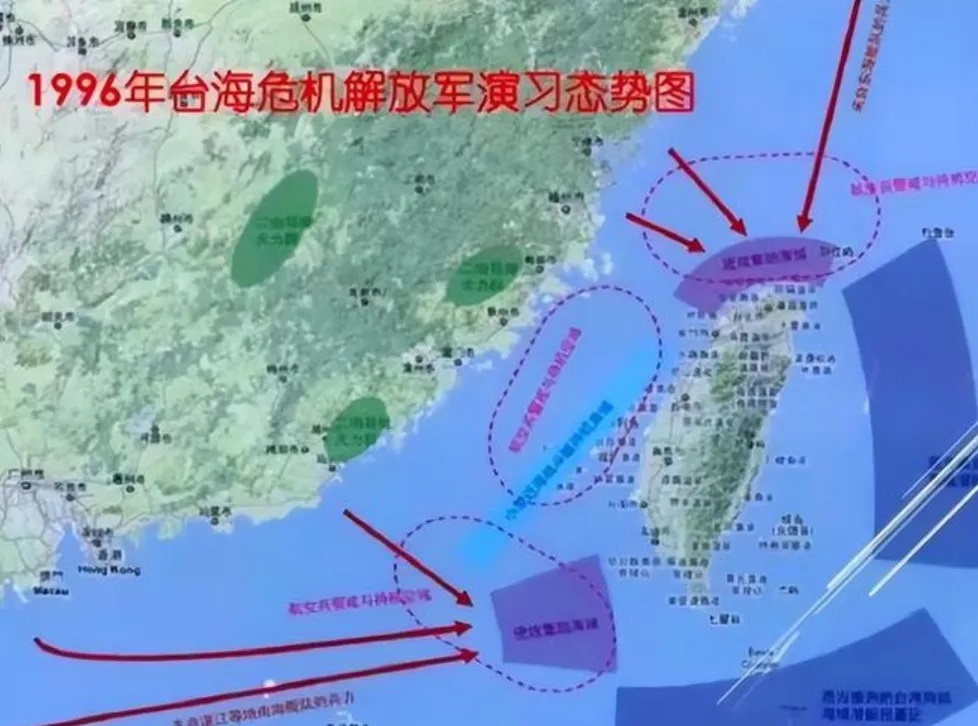
\includegraphics[width=9cm]{2024-08-18-001.jpg}
\end{figure}

中国海军的力量远远弱于和自己对峙的美国海军,而海军不比陆军,在茫茫大海上人的意志力能发挥的空间相当有限。

\zd{射程不够就是打不到,火力不够就是无法击破铁甲防御,船被打沉了就是会沉,意志力再强都无法改变这个客观事实。}

而如果当时的中国海军和美国两大航母战斗群开战,那美国航母战斗群可以零损伤击沉所有中国海军。

不是哪一方这么说,而是全球几乎所有的军棋推演都只能推出这个结果,双方海军的实力差距过于离谱。

\zd{不是说1996年的中国海军怎么做才能打赢美国航母战斗群,而是连给航母战斗群造成1滴血的损伤都难。}

当时的中国甚至连GPS都依赖于美国提供,美国把GPS导航一关,就连路基导弹都能变成瞎子,而美军航母可以从数百公里外肆无忌惮的打击中国船只,解放军连靠近开一炮都不可能。

1996年,美国的军费开支是2657亿美元,中国的军费开支是86.66亿美元,台湾地区的军费开支是85亿美元。

中国大陆的开支不仅只有美国的零头,甚至只比台湾地区略多一点点。

在这个基础上,中国大陆的军费还主要投入到陆军和战略导弹部队上,留给海军的很少,而美国是两洋国家,海军为立国之基,吃了军费的大头。

从这个军费差距,你就能感受到中美两国在1996年的时候海军的实力差距。

\zd{中国海军不仅投入弱,底子还差,1950年3月新任的海军司令萧劲光视察威海时甚至都没有船可以坐,只能租渔民的渔船渡海。}

\begin{figure}[H]
    \centering
    
\includegraphics[width=9cm]{2024-08-18-002.jpg}
\end{figure}

所以1996年的时候中国海军压根没有实力去和美国航母战斗群对峙,这个是明牌,所有人都知道。

\zd{但台湾是中国的底线,打击台独势力是中国解放军的使命,所以哪怕根本就没有那个实力,在台海军演并和美国两大航母战斗群对峙的任务中国海军也必须完成。}

\zd{根本没有实力完成的任务,中国海军怎么完成?}

1996年,在美国两大航母战斗群驶入台湾海域的同时,中国海军紧急征调了2000艘渔船,把陆军的大炮和坦克拉上渔船固定,派这些“军舰”去和美国航母战斗群对峙。

\begin{figure}[H]
    \centering
    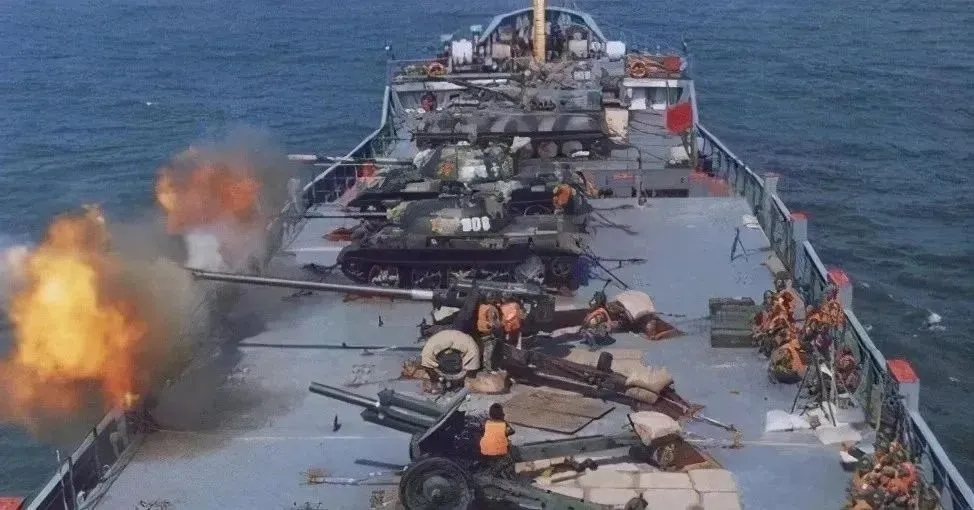
\includegraphics[width=9cm]{2024-08-18-003.jpg}
\end{figure}

\zd{中国海军不仅把坦克大炮拉上了渔船,还在台湾海峡大规模火力射击,拍下照片展示给全球看,形成了在全球军事史上独一份的奇观。}

中国坦克在渔船上射击的摸样,是下面这样的。

\begin{figure}[H]
    \centering
    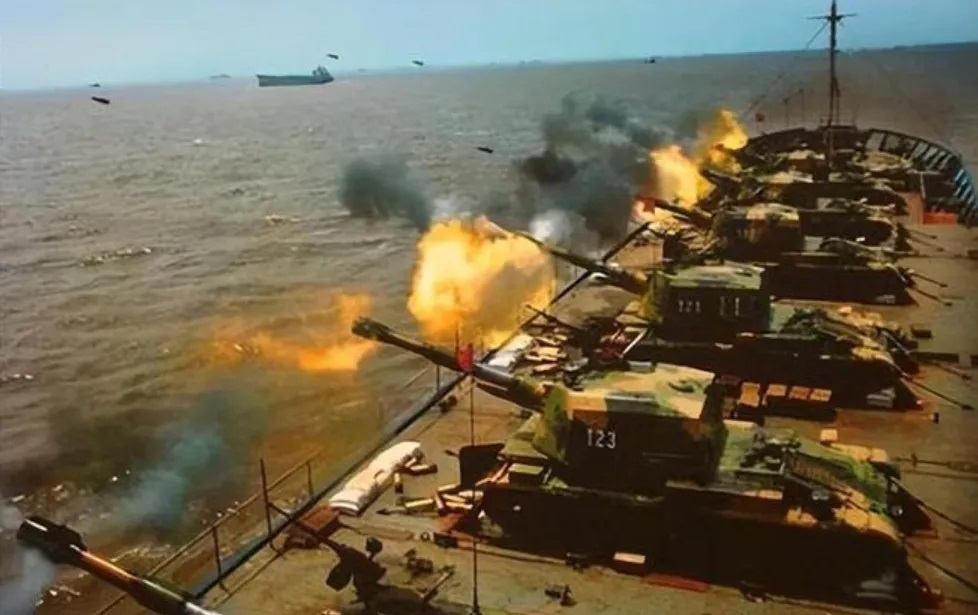
\includegraphics[width=9cm]{2024-08-18-004.jpg}
\end{figure}

坦克大炮上渔船这个事,从军事上来说没有任何意义,属于纯粹的送死。

陆军的坦克大炮是为了陆战准备的,是具备在陆地上快速行军能力的,所以重量和口径都极小。

而军舰可以在海洋上行军,不需要考虑行军困难问题,所以可以拥有极为厚重的坚甲以及大到离谱的口径。

别说战列舰那种巨无霸,就算是轻型军舰都不是坦克能对抗的。

1943年意大利萨莱诺登陆战中,为了阻挡美军登陆,德军13装甲师派出了18辆虎式坦克,43辆4号坦克阻挡美军2艘驱逐舰和一艘巡洋舰。

这些驱逐舰和巡洋舰火力很弱,仅仅只有舰载主炮,而虎式坦克为二战时人类最强坦克,拥有高达100毫米的正面装甲。

虎式坦克同时也拥有二战时人类最强大的坦克主炮,但口径仅为88毫米。

这个口径的坦克炮让虎式坦克的射程仅有几公里,且即便命中也无法击穿军舰的护甲。

而美国驱逐舰的射程接近20公里,且只需一炮就能让虎式坦克变成零件。

因为舰载主炮发射出去的炮弹,光弹头就很重,哪怕不爆炸,仅凭动能都可以把虎式坦克砸成重伤。

如果直接命中,那虎式坦克就会变成下面这样的零件状态。

\begin{figure}[H]
    \centering
    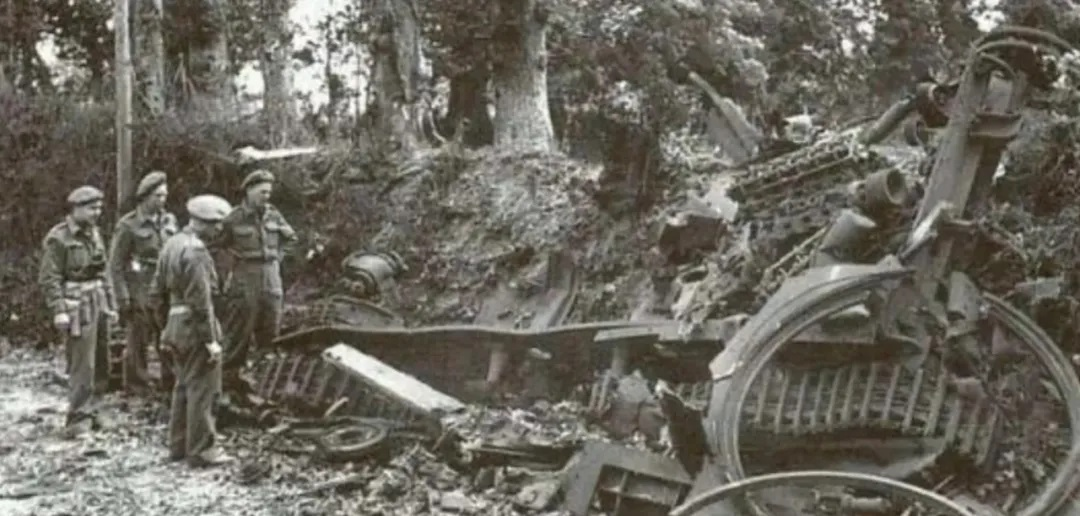
\includegraphics[width=9cm]{2024-08-18-005.jpg}
\end{figure}

这场战斗被美军记载为“拍蚊子”战斗,仅用20分钟就击毁了德军29辆坦克,美国军舰毫发无伤,登陆部队仅6人轻伤,德军阻止美军登陆的企图完败。

当年德国虎式坦克和美国军舰战斗的地点好歹是陆地上,而如今中国解放军直接把坦克搬上了渔船。

那甚至都不需要挨个打坦克,只需要对准渔船来一炮,全船的坦克都得下海喂鱼,而解放军坦克的主炮连射到美国军舰边上打个水花都不可能。

把这么多坦克大炮拉上渔船和美国航母战斗群对峙后,军棋推演的结果依然是美国零损伤歼灭中国海军全部,结果没有任何差异。

\zd{既然这么做纯粹是送死,没有任何军事意义,为什么中国海军还要这么做?}

因为这么做可以向美国展示我们不怕死的决心。

\zd{当时全军上下都知道如果中美爆发海战,所有和美国航母战斗群对峙的海军都不可能活下来,所以海军将士在出海前都已经写下了遗书,此去就没打算活着回来,是抱着必死的决心和美国航母战斗群对峙的。}

\zd{跟着坦克大炮上渔船的陆军将士,也都写了遗书,也没打算活着回来,因为只要真打起来那自己是肯定回不来的。}

\zd{但这么做并不是平白无故的送死,而是给美军展示自己到底有多不怕死,为了维护对台湾的主权愿意付出多大牺牲。}

美军航母战斗群确实可以无损把我们的船都打沉在台湾海域,但如果我们中国这么多军舰,这么多士兵,这么多坦克大炮全部沉在了海上。

无论何人主政,中国都必须反击,而当时的中国唯一能对美国造出实质性损伤的反击手段只有战略核武器。

所以如果1996年美国航母战斗群敢于击沉我们拉上渔船的坦克大炮,那就直接是全球核战。

我们把这么多写下遗书的将士送上了渔船,就是用这巨大的牺牲来给美军展示我们的决心,维护台湾主权的决心,以及巨大牺牲后启动核战同归于尽的决心。

\zd{所以坦克大炮上渔船是人类奇观,因为这一招只有中国在1996年那种环境下会用。}

\zd{这种没有任何军事价值的自杀行为,海军强国不会用,海军弱国也不会用,任何国家都不会用这一招,没有任何意义,但对于拥有战略核武器但海军奇弱无比的中国来说,刚好合适。}

美军丝毫不惧怕解放军拉上渔船的坦克和大炮,但惧怕中国战略洲际导弹上携带的氢弹,所以在中国解放军这种无惧牺牲,宁愿都死在海上也绝不退缩的精神意志展示后,美军怂了。

经过谈判,可以零损伤歼灭中国海军全部的美军两大航母战斗群主动后撤270海里,而解放军逐渐停止了相关军事演习,战争的阴影逐渐消散,96台海危机解除。

中国的核武器和无惧牺牲的精神,让我们在1996年守住了台湾主权的底线,但这种同归于尽的自杀式威胁是当时国力太弱时无奈的选择,没有人想一直这样,而且在96事件发生后,因为海军实力确实不能控制台湾海域,台独势力从此开始抬头并蔓延到今天。

\zd{解放军不怕死,但没人不想正面击败美国航母战斗群,96年那种无奈的选择没人想再来一次。}

中国海军司令员,解放军上将刘华清曾经说过:

\yh{“中国不建航母,我死不瞑目!” }

可惜直到刘华清上将去世,中国都没有建出航母,因为国力实在是不允许。

\begin{figure}[H]
    \centering
    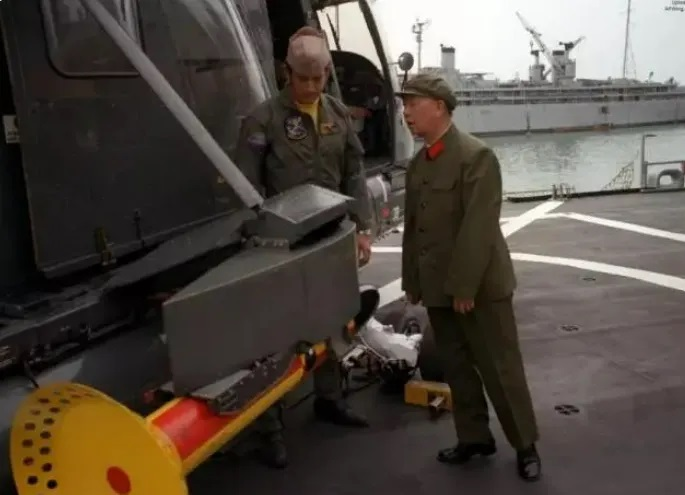
\includegraphics[width=9cm]{2024-08-18-006.jpg}
\end{figure}

\zd{海军太贵了,太烧钱了,国家经济没有发展到一定地步是真的建不起海军。}

2000年,中国北斗系统首次建成,路基导弹终于拥有了威胁美军航母的能力。

就4年时间,一眨眼的功夫,美国还没想明白怎么解决中国海军这种自杀性对峙的时候,中国就集中资源抢先解决了最卡脖子的问题,给路基反舰导弹安上了眼睛。

从这一刻开始,中国再也不需要坦克大炮上渔船,拿命去威胁美军航母了,只需要不断提升路基反舰导弹的射程就行了。

反舰导弹射程500公里,美军航母就不敢靠近台湾海峡500公里。

反舰导弹射程1000公里,美军航母就不敢靠近台湾海峡1000公里。

所以中国才对研发反舰导弹那么有兴趣,集中全国资源研发出了人类最强的反舰导弹。

\zd{中国东风-21D的最大射程已经达到了2500公里,最高可达10倍音速,这数据堪称丧心病狂,简直是为了打航母而打航母,倾尽一切只为了在最远距离上弄死航母。}

\zd{全人类都没有数据这么变态的反舰导弹,因为不需要,有这个动力砸钱研究这玩意的唯有中国,而这个动力是美军航母在1996年给的。}

而路基反舰导弹只能防御,进攻还是只能依靠海军,但进攻才是最好的防御。

2012年,中国航母首次下水,中国首次拥有了自己的舰载航空兵。

\begin{figure}[H]
    \centering
    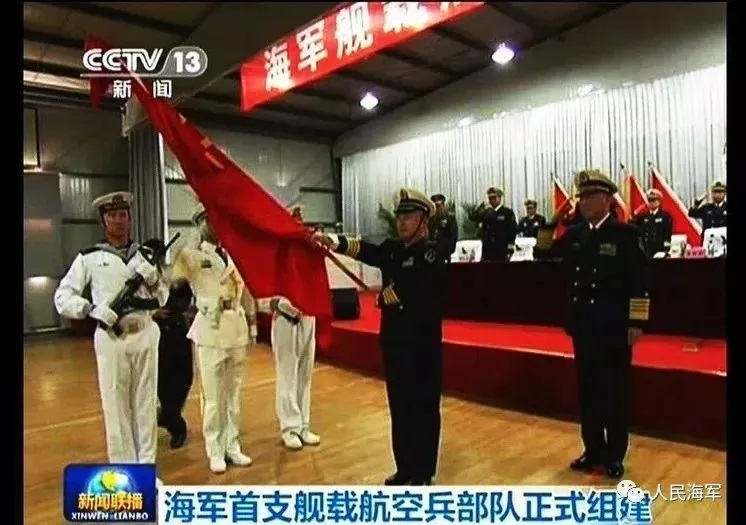
\includegraphics[width=9cm]{2024-08-18-007.jpg}
\end{figure}

2023年,中国已经拥有了3个航母战斗群。

\begin{figure}[H]
    \centering
    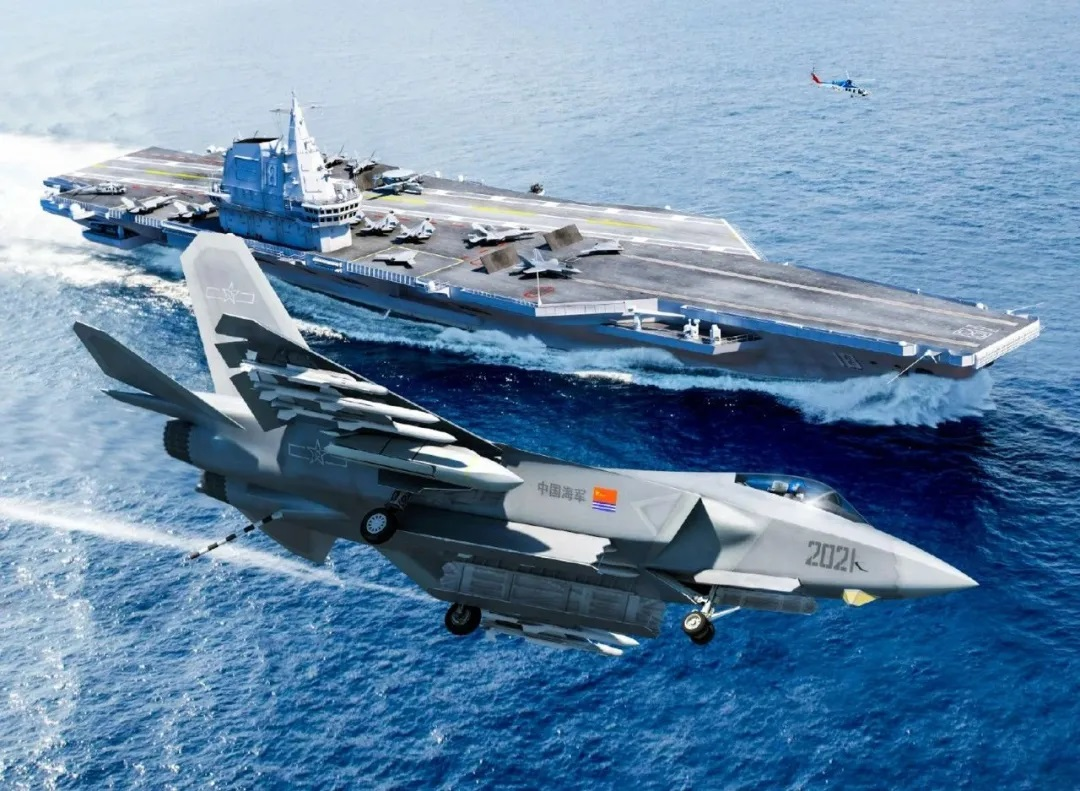
\includegraphics[width=9cm]{2024-08-18-008.jpg}
\end{figure}

2012年,中国首艘052C型导弹驱逐舰下水,号称中华神盾,是解放军最先进的主战舰艇,这么现先进的宙斯盾级驱逐舰当时中国只有2艘。

而美国共有90艘“宙斯盾”战舰,其中“阿利伯克”66艘,“提康德罗加”22艘,“朱姆沃尔特”2艘。

在美国国力最强大的1994年,一年时间美国就下水了6艘宙斯盾驱逐舰。

但是中国强大的时候,曾经被人拍到过5艘052D导弹驱逐舰同框建造,在同一个造船厂里批量化生产。

\begin{figure}[H]
    \centering
    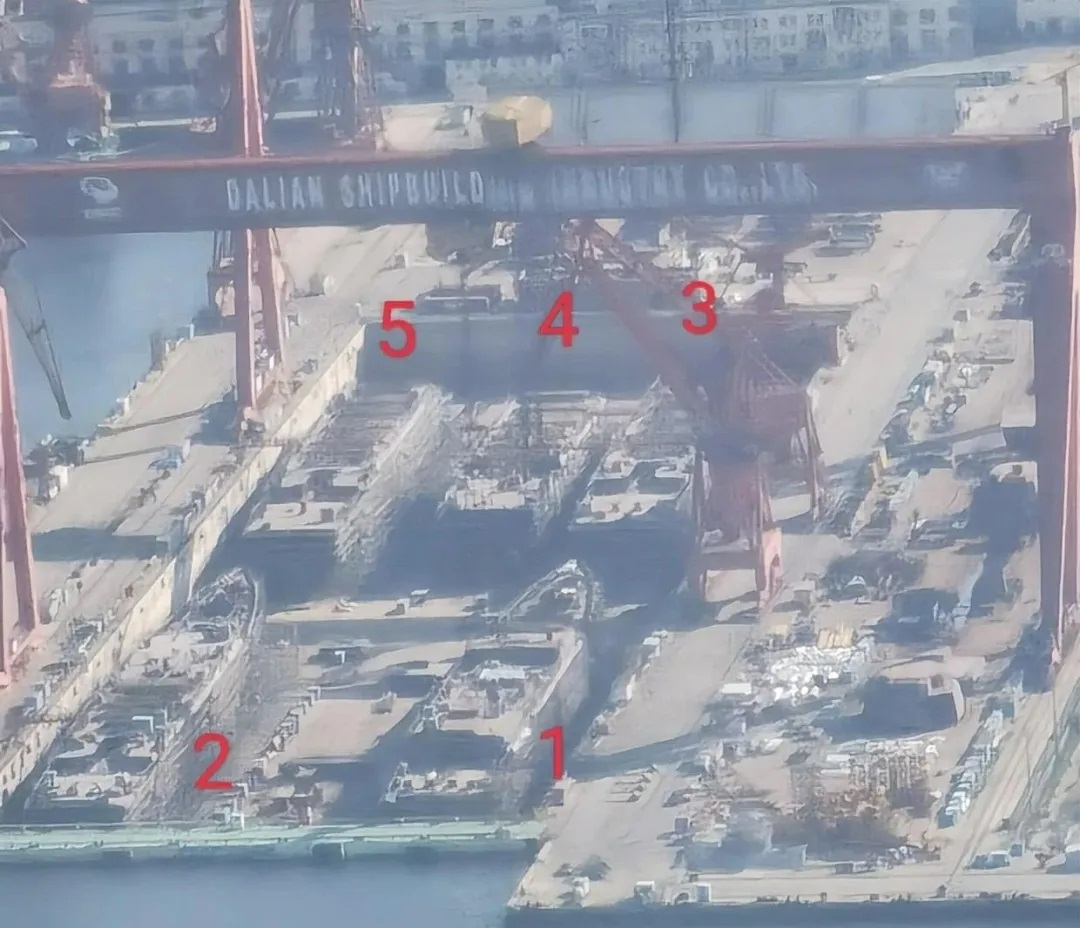
\includegraphics[width=9cm]{2024-08-18-009.jpg}
\end{figure}

这一幕,震惊世界。

\begin{figure}[H]
    \centering
    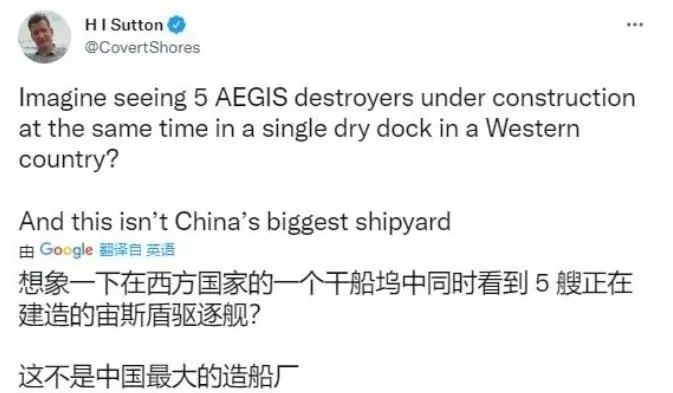
\includegraphics[width=9cm]{2024-08-18-010.jpg}
\end{figure}

2019年,中国一年内下水了8艘052D级和2艘055级导弹驱逐舰,打破了美国1994年的记录。

这个速度,被人称之为下饺子。

造船业的工业能力,目前的中国一骑绝尘。

\begin{figure}[H]
    \centering
    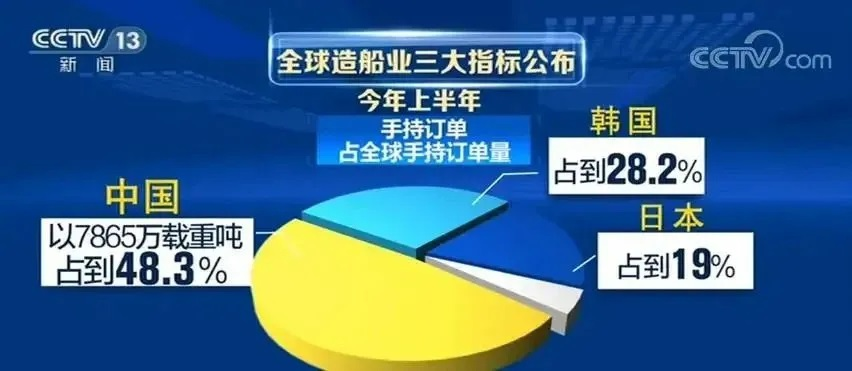
\includegraphics[width=9cm]{2024-08-18-011.jpg}
\end{figure}

截止2020年末,中国的盾舰数量已经超过了40艘,达到了美国存量盾舰的一半。

2021年,中国下水8艘盾舰。

2022年,中国下水9艘盾舰。

你要知道世界第三大海军英国全国所有的盾舰总共才6艘。

而美国的盾舰数量虽然多,但很多都是二三十年前建造的老产品,战斗性能上已经落后中国导弹驱逐舰不止一代,而且美国的海军需要分布全球镇压,不能全部拿来对付中国。

所以2023年的中国海军再也不用坦克大炮上舰了,美国试图搞黄海军演来挑事的时候,我们看美军航母战斗群没来还颇为可惜,派山东号航空母舰带着一群盾舰去找关岛基地找美军航母聊天去了。

\zd{美国航母退缩后,本来猖獗的台独势力立刻就萎了,蔡英文公开发言和平对话才是解决两岸问题的正确道路,战争不是选项,热爱和平之心简直是令人刮目相看。}

\begin{figure}[H]
    \centering
    
\includegraphics[width=9cm]{2024-08-18-012.jpg}
\end{figure}

现在是和平时代,有核武的年代没有大国敢于轻易发动战争,为什么还要砸那么多钱发展海军,这不是劳民伤财吗?

\zd{因为能不战而屈人之兵,才是真正的和平。}

\zd{世界上再也没有国家的海军会把坦克大炮拉上渔船了,这一幕将成为千古绝唱。}

\end{document}

